
\begin{frame}
	\frametitle{Alternative requirements}
	\begin{columns}
		\begin{column}{0.5\textwidth}
				\begin{itemize}[<+->]
				\item Place requirements directly on one power plant.
				\includegraphics<1>{./pictures/sys.tikz}
				\includegraphics<1>{./pictures/req_sys.tikz}
				\item We already have an estimate of $G_1(s)$.
				\item We need to find $S(s)$
			\end{itemize}
		\end{column}
		\begin{column}{0.5\textwidth}
			\begin{figure}
				\includegraphics<2>[width=\textwidth]{./pictures/PMU_bode.tikz}
			\end{figure}
		\end{column}
	\end{columns}
\end{frame}
\begin{frame}
	\frametitle{Estimating $S(s)$}
	\begin{itemize}[<+->]
		\item
		\begin{equation} 
			G_1(s) = G_J(s)S(s)
		\end{equation}
		\item
		\begin{equation}
			G_J(s) = \frac{1}{2Hs+K_d}
		\end{equation}
		\item
		\begin{equation}
			2H>>K_d
		\end{equation}
		\item
		\begin{equation}
			S(s) \approx 2HsG_1(s)
		\end{equation}
		\item Need to estimate $H$
	\end{itemize}
\end{frame}
\begin{frame}
	\frametitle{Estimating $H$}
	\begin{figure}
			\includegraphics[width=0.9\textwidth]{./pictures/transf_comp.tikz}
	\end{figure}
\end{frame}
\begin{frame}
	\frametitle{Dataset from Statkraft}
	\begin{itemize}[<+->]
		\item Norway's biggest power producers.
		\item They performed the tests from the draft requirements
		\item By chance I had PMU measurements from the same plant.
		\end{itemize}
		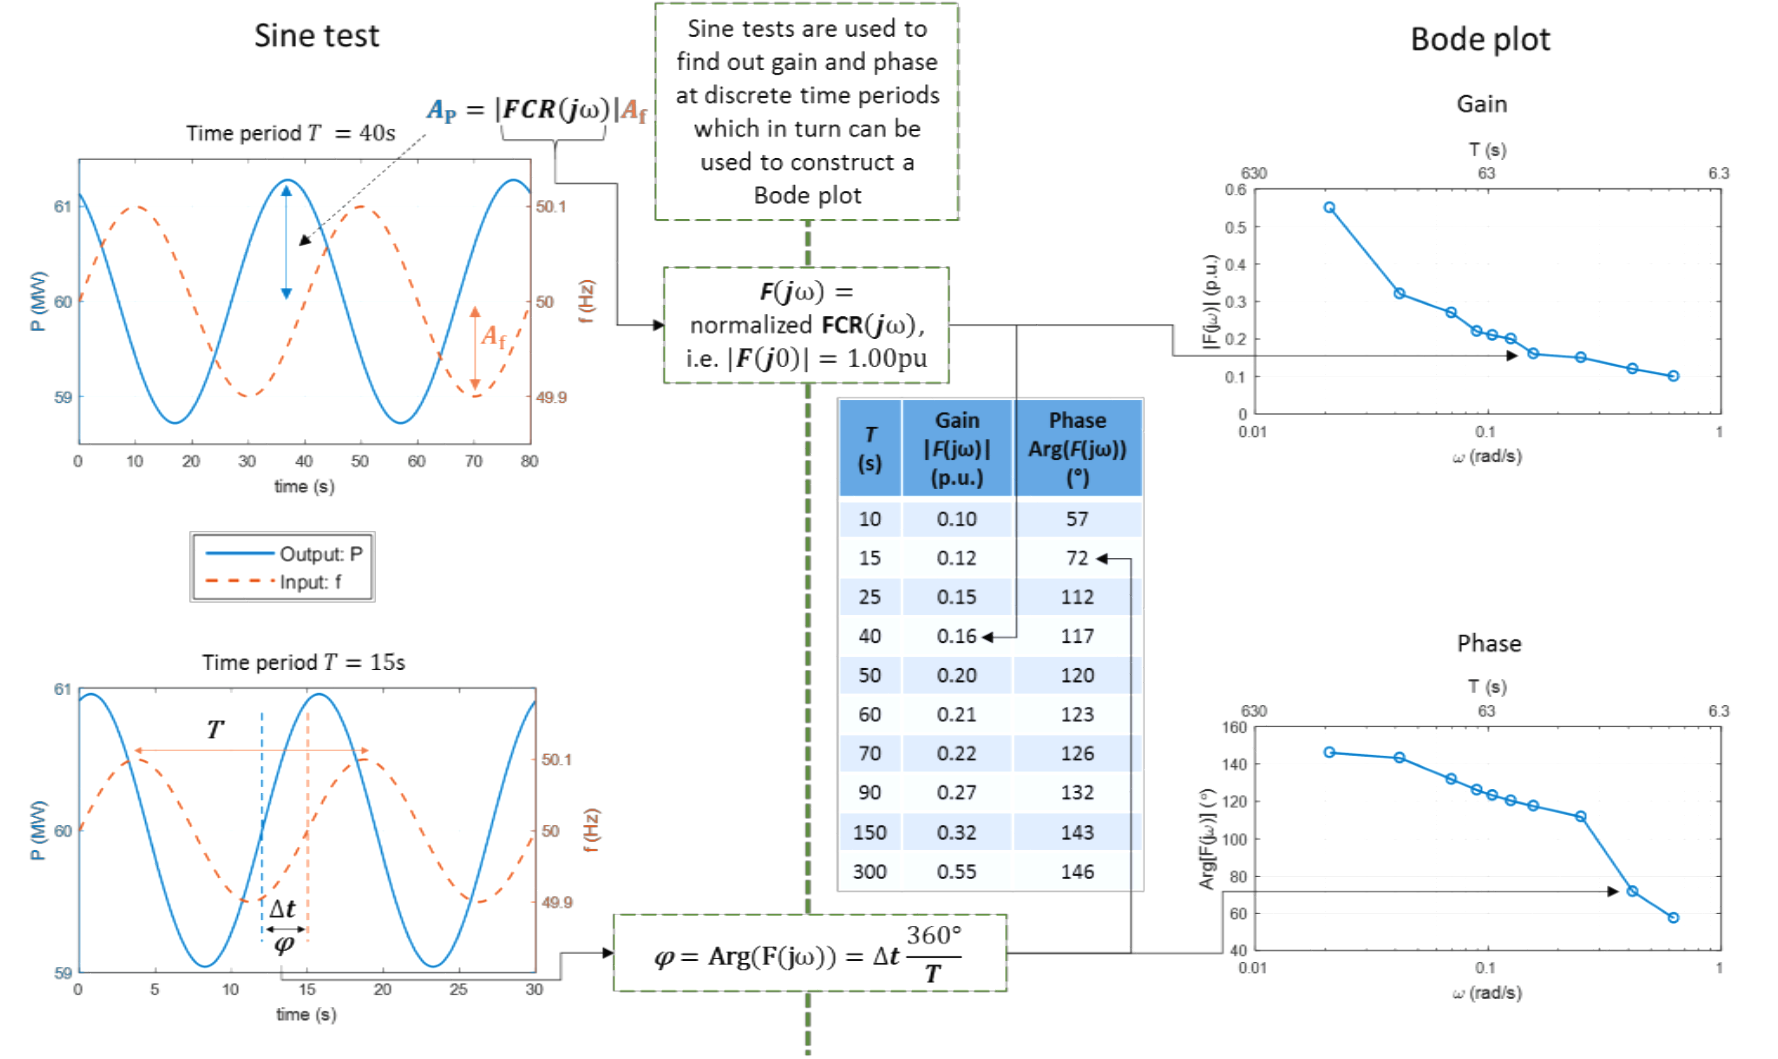
\includegraphics[width=0.8\textwidth]{./pictures/tests.png}
\end{frame}
\begin{frame}
	\frametitle{Can the industry proposed tests be done easier?}
	\begin{figure}
		\includegraphics<1->[width=0.6\textwidth]{./pictures/aura_signals.tikz}
	\end{figure}
	\begin{figure}
		\includegraphics<1>[width=0.6\textwidth]{./pictures/frd.tikz}
		\includegraphics<2>[width=0.6\textwidth]{./pictures/frd_vs_bj.tikz}
	\end{figure}
\end{frame}
\begin{frame}
	\frametitle{Datasets used}
	\begin{figure}
			\includegraphics[width=0.8\textwidth]{./pictures/signals_step.tikz}
	\end{figure}
\end{frame}
\begin{frame}
	\frametitle{Estimated sensitivity functions}
		\begin{figure}[tb]
			\includegraphics[width=0.8\textwidth]{./pictures/S_aura.tikz}
		\end{figure}
\end{frame}
\begin{frame}
	\frametitle{Estimated $G_1(s)$}
		\begin{figure}[tb]
			\includegraphics[width=0.8\textwidth]{./pictures/G1_aura.tikz}
		\end{figure}
\end{frame}
\begin{frame}
\begin{frame}
	\frametitle{Identification cases}
	\begin{enumerate}
		\item \textbf{Case 1} Normal operation and speed feedback.
		\item \textbf{Case 2} Normal operation, speed feedback and PMU.
		\item \textbf{Case 3} Normal operation, frequency feedback and PMU.
		\item \textbf{Case 4} Open loop operation. 
	\end{enumerate}
	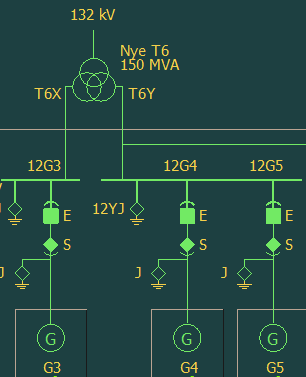
\includegraphics{./pictures/plant.tikz}
\end{frame}
\begin{frame}
	\frametitle{Test the different cases}
	\begin{figure}
		\includegraphics<1>[width=0.9\textwidth]{./pictures/G0_sim.tikz}
		\includegraphics<2>[width=0.9\textwidth]{./pictures/G_req_sim.tikz}
	\end{figure}
\end{frame}
	\frametitle{More detailed power plant model}
	\begin{figure}
		\includegraphics{./pictures/PID.tikz}
	\begin{figure}
		\includegraphics{./pictures/governor.tikz}
	\end{figure}
	\end{figure}
	\begin{figure}
		\includegraphics{./pictures/turbine.tikz}
	\end{figure}
\end{frame}
\begin{frame}
	\frametitle{Test backlash}
	\begin{figure}
		\includegraphics[width=0.9\textwidth]{./pictures/backlash.tikz}
	\end{figure}
\end{frame}
\begin{frame}
	\frametitle{Test deadband}
	\begin{figure}
		\includegraphics[width=0.9\textwidth]{./pictures/deadband.tikz}
	\end{figure}
\end{frame}
\begin{frame}
	\frametitle{Test frequency assumption}
	\begin{figure}
		\includegraphics[width=0.9\textwidth]{./pictures/reactances.tikz}
	\end{figure}
\end{frame}
%\begin{frame}
		%\frametitle{Sensitivity function $S(s)$}
	%\begin{figure}
		%\includegraphics[width=0.9\textwidth]{./pictures/S_sim.tikz}
	%\end{figure}
%\end{frame}
%\begin{frame}
		%\frametitle{Disturbance rejection function $G_1(s)$}
	%\begin{figure}
		%\includegraphics[width=0.9\textwidth]{./pictures/G0_req_sim.tikz}
	%\end{figure}
%\end{frame}
\begin{frame}
	\frametitle{Comparison of stability margins}
			\begin{tabular}{c c c}
			\toprule
			Method & Median & Root mean square error (RMSE) \\
			$\max |S(j\Omega)|$ & $1.84$ & $0$ \\
			$\max |S(e^{j\Omega},\hat{\theta})|$, Case 1 & $1.84$ & $0.25$ \\
			$\max |S(e^{j\Omega},\hat{\theta})|$, Case 2 & $1.75$ & $0.34$ \\
			$\max |S(e^{j\Omega},\hat{\theta})|$, Case 3 & $1.74$ & $0.39$ \\
			$\max |S_{\min}(e^{j\Omega},\hat{\theta})|$ & $1.66$ & $0.25$ \\
			\bottomrule
	\end{tabular}
\end{frame}
\begin{frame}
	\frametitle{Comparison of estimated inertias}
	\begin{tabular}{c c c}
			\toprule
			Case & Median & RMSE \\
			Actual & $3.5$ & $0$ \\
			Case 1& $3.40$ & $0.46$ \\
			Case 2 & $3.33$ & $0.40$ \\
			Case 3 & $3.27$ & $0.43$ \\
			\bottomrule
	\end{tabular}
\end{frame}
